\documentclass[pre,twocolumn,superscriptaddress,nofootinbib]{revtex4-2}
\usepackage{amsmath,amssymb,amsthm}
\usepackage{placeins}
\usepackage{graphicx}
\usepackage{booktabs}
\usepackage[colorlinks=true,allcolors=blue]{hyperref}

\newtheorem{theorem}{Theorem}
\newtheorem{lemma}{Lemma}
\newtheorem{proposition}{Proposition}
\newtheorem{conjecture}{Conjecture}
\newcommand{\Aex}{\langle A_{\rm ex}\rangle}
\newcommand{\nd}{n_c^{\rm disk}}
\newcommand{\RepoURL}{https://github.com/toyamataiyo03-cpu/k-star-percolation}
\newcommand{\ContribEn}{T. Toyama initiated and directed the project (choice of research area, priority on novelty, the decision to seek a mathematical proof and to test the conjectured prefactor numerically), checked the results, and takes full responsibility for the content.}
\newcommand{\ContribJa}{遠山は研究を発起・主導し（分野の選択，新規性の重視，数学的証明を目指す判断，予想の係数を数値で検証する判断），結果を確認し，内容に全責任を負う。}


\begin{document}

\title{Continuum percolation of $k$-armed stars in two dimensions:\\ a $k^{-2/3}$ approach to the disk limit}

\author{Taiyo Toyama}
\affiliation{Hokkaido Asahikawa Higashi High School, Asahikawa, Hokkaido, Japan}
\email{toyamataiyo03@gmail.com}


\begin{abstract}
We study two-dimensional continuum percolation of randomly placed, randomly oriented $k$-armed stars---$k$ zero-width segments of length $a$ emanating at equal angles from a common centre---which interpolate between sticks ($k=2$) and disks ($k\to\infty$).
Monte Carlo simulations with wrapping-probability estimators give the critical number density $n_c$ for $2\le k\le 512$, with relative precision $10^{-4}$ for $k\ge 64$, reproducing the known stick value.
Analytically, we show that the contact probability of two stars equals the area of a contact set modulo the square lattice $(2\pi/k)\mathbb{Z}^2$ of arm-angle pairs, and we bound it from both sides.
This yields a proof that the mean excluded area falls short of the disk value by
$Ck^{-2/3}-C'k^{-4/3}+O(k^{-2})$ with $C=\tfrac{18}{5}2^{1/3}\pi^{5/3}$ and $C'=\tfrac{36}{7}2^{-1/3}\pi^{7/3}$; the error term is made explicit ($\le 2396/k^2$ for $k\ge106$) by a computer-assisted argument in ball arithmetic.
Showing that stars closer than $2a(1-\varepsilon_1)$ always touch, we prove $\nd\le n_c(k)\le \nd(1-\varepsilon_1)^{-2}$ with $\varepsilon_1\simeq(\pi/ck)^{2/3}$, i.e.\ convergence at rate $O(k^{-2/3})$ without using the value of the disk threshold.
A first-order perturbative argument predicts $(n_c-\nd)a^2\simeq0.873\,k^{-2/3}$, which the simulations confirm to within $0.5\%$ at $k=512$.
The critical mean number of contacts varies from $3.59$ (sticks) to $4.51$ (disks), so excluded-area invariance fails for branched objects.
\end{abstract}

\maketitle

\section{Introduction}
Continuum percolation---the onset of long-range connectivity among randomly placed, mutually overlapping objects---models conductive composites, nanowire networks and porous media~\cite{Stauffer1994,Balberg1984}.
In two dimensions precise thresholds are known for disks, squares and sticks~\cite{Mertens2012,Baker2002,Pike1974} and for rectangles~\cite{Li2013}.
A widely used organising principle is the excluded-area heuristic of Balberg \textit{et al.}~\cite{Balberg1984}: if $\Aex$ is the orientation-averaged area of relative positions at which two objects touch, the critical mean number of contacts
\begin{equation}
B_c=n_c\Aex \label{eq:Bc}
\end{equation}
is approximately shape independent.

Branched particles such as tetrapod nanocrystals~\cite{Manna2003} motivate the study of non-convex, branched shapes.
The simplest idealisation is the regular $k$-armed star: $k$ segments of length $a$ from a common centre at angles $2\pi/k$ apart (Fig.~\ref{fig:stars}).
The family interpolates between sticks of length $2a$ ($k=2$) and disks of radius $a$ ($k\to\infty$).
Excluded areas of ``star lines'' have been computed as functions of relative orientation for hard-particle phase behaviour~\cite{Geigenfeind2019}, and the shape dependence of critical intensities is understood rigorously for convex grains~\cite{RoyTanemura2002}.
To our knowledge, however, percolation thresholds of stars with $k\ge3$, and the rate at which they approach the disk value, have not been reported.

This paper (i) determines $n_c(k)$ numerically for $2\le k\le512$, (ii) proves that the excluded-area deficit decays as $k^{-2/3}$ with explicit constants, (iii) proves that $n_c(k)$ converges to the disk threshold at rate $O(k^{-2/3})$, and (iv) tests a conjectured prefactor and the excluded-area invariance.


\section{Model and numerical method}
Star centres are placed uniformly at random in an $L\times L$ periodic box, each with an independent uniform orientation in $[0,2\pi/k)$.
Two stars are connected if any arm of one intersects any arm of the other.
Lengths are measured in units of $2a$ and densities are reported as $n_ca^2$.
The reference values are $n_ca^2=5.6372858/4=1.4093215$ for $k=2$ and $\nd a^2=1.12808737/\pi=0.3590819$ for disks~\cite{Mertens2012}.

We use the Newman--Ziff union--find algorithm~\cite{NewmanZiff2001} in its continuum form~\cite{Mertens2012}: stars are added one by one, neighbours are found with a cell list of side $2a$, and displacement vectors stored in the union--find tree detect wrapping clusters.
For each sample we record the number of stars at which a cluster first wraps horizontally ($N_h$) and in either direction ($N_e$).
The grand-canonical wrapping probability is $R(n)=\langle \Pr[\mathrm{Pois}(nL^2)\ge N]\rangle$, and $n_c(L)$ solves $R(n)=R^*$ with the exact torus values $R_h^*=0.521058$ and $R_e^*=0.690474$~\cite{Pinson1994}.
For $k\le 48$ we used $L=16$--$128$ ($2\times10^4$ to $10^3$ samples) and extrapolated linearly in $L^{-2}$; for $k\ge64$ we used $2\times10^5$ samples at $L=64$ and $4\times10^4$ at $L=128$, whose results agree within errors.
Errors are bootstrap estimates.

For large $k$ we test contacts in $O(k)$ rather than $O(k^2)$ operations: each arm of one star that can reach the other star's disk is clipped to that disk, and the arms of the second star that hit the clipped piece are those whose angles lie in the angular interval it subtends---an $O(1)$ check because the arm angles form a lattice.
This test agreed with brute force on $1.3\times10^6$ random configurations.
The code uses Numba~\cite{Numba}.

\begin{figure*}[tb]
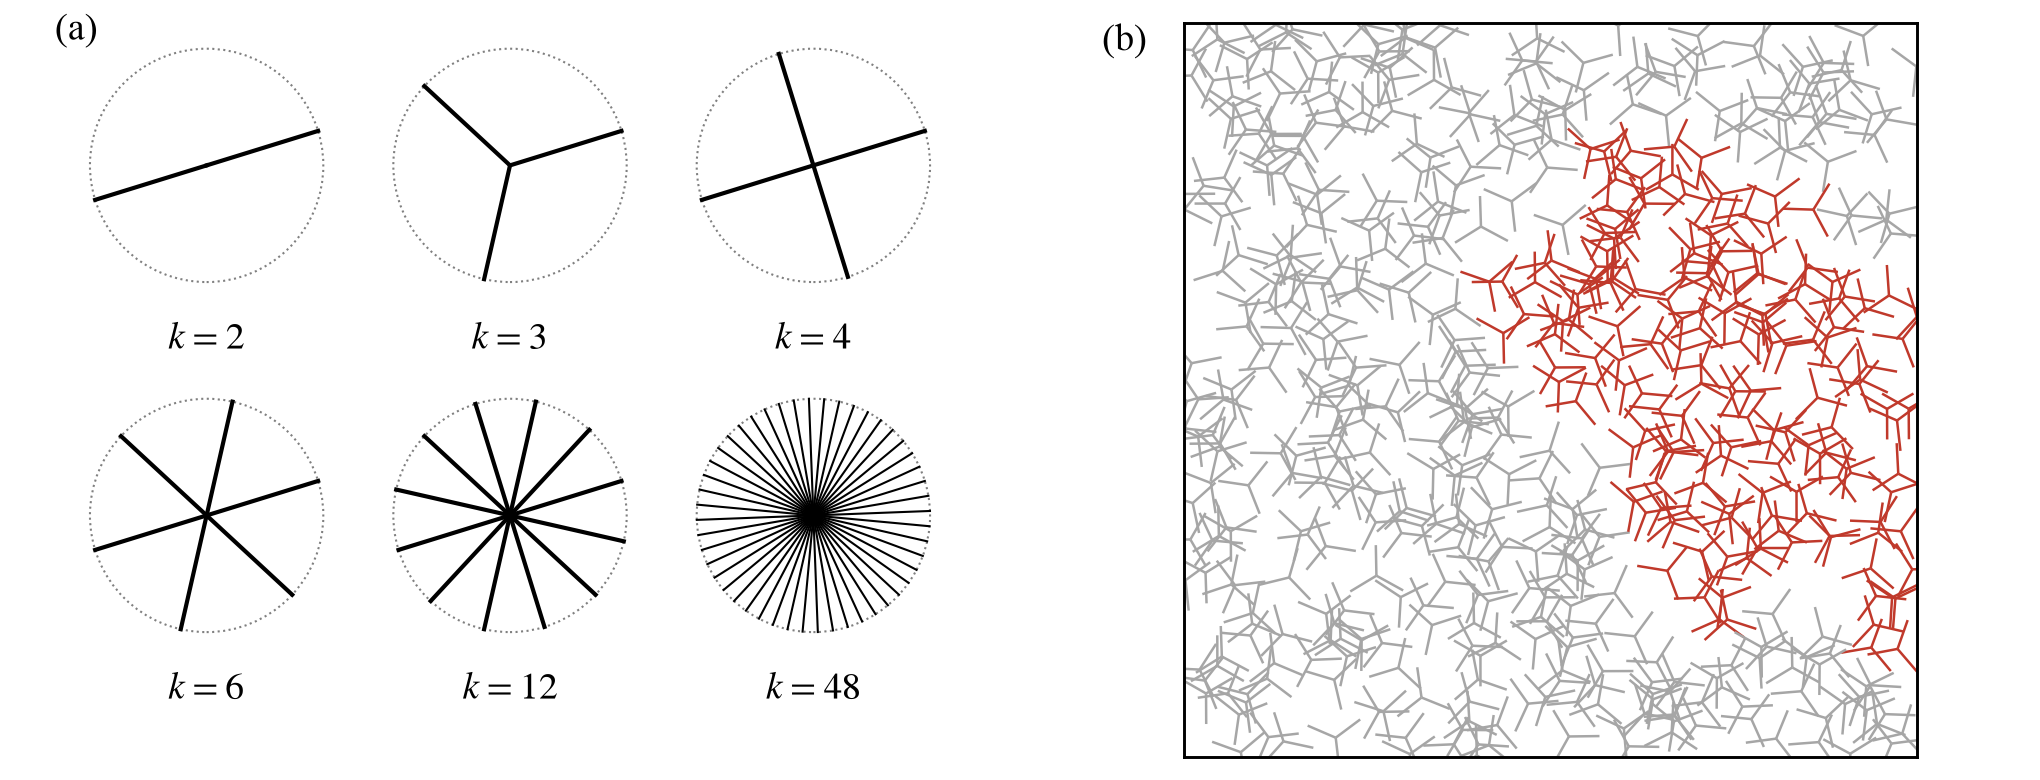
\includegraphics[width=0.86\textwidth]{fig1_stars.png}
\caption{(a) $k$-armed stars (dotted circle: radius $a$). (b) Stars with $k=3$ near the threshold in a $12\times12$ region (units of $2a$); red: largest cluster.}
\label{fig:stars}
\end{figure*}

\section{Contact condition and lattice representation}
Set $a=1$, $h=2\pi/k$ and $r=2(1-\varepsilon)$ for the centre distance.
Let $D(k)=4\pi-\Aex=8\pi\int_0^1(1-\varepsilon)\,[1-P_k(\varepsilon)]\,d\varepsilon$, where $P_k$ is the contact probability at distance $r$.

\begin{lemma}[two arms]
Let the arm of star A make angle $\alpha$ with the segment AB and the arm of star B make angle $\beta$ with BA, with the same side counted positive.
For $r>1$ the arms intersect if and only if $\alpha,\beta$ have the same sign and
\begin{equation}
r\sin|\beta|\le\sin(|\alpha|+|\beta|),\qquad r\sin|\alpha|\le\sin(|\alpha|+|\beta|).\label{eq:contact}
\end{equation}
\end{lemma}
\noindent This follows from the law of sines in the triangle formed by the two centres and the intersection point.
Let $S_r$ be the set of $(\alpha,\beta)$ with $\alpha,\beta>0$ satisfying~\eqref{eq:contact} and $T_r=S_r\cup(-S_r)$.
Because~\eqref{eq:contact} weakens as $r$ decreases, $S_r\supseteq S_{r'}$ for $r<r'$.

\begin{lemma}[lattice representation]
The arm-angle pairs form the shifted lattice $s+h\mathbb{Z}^2$ with $s$ uniform on $[0,h)^2$, hence
\begin{equation}
P_k(r)=\bigl|T_r \bmod h\mathbb{Z}^2\bigr|/h^2 .\label{eq:lattice}
\end{equation}
\end{lemma}

In coordinates $u=(\alpha+\beta)/2$, $\delta=\alpha-\beta$ (unit Jacobian) the lattice is generated by $(h,0)$ and $(h/2,h)$, and
\begin{equation}
S_r=\{|\delta|\le g_\varepsilon(u)\},\quad g_\varepsilon(u)=2\Bigl[\arcsin\frac{\sin2u}{2(1-\varepsilon)}-u\Bigr],\label{eq:g}
\end{equation}
supported on $0<u\le\arccos(1-\varepsilon)$.
With $u=\sqrt\varepsilon\,v$ one finds $g_\varepsilon=\varepsilon^{3/2}[v(2-v^2)+\varepsilon v(2-v^2/3-v^4/4)+O(\varepsilon^2)]$, so the half-width of $S_r$ in $\delta$ is
\begin{equation}
\delta_{\max}(\varepsilon)=c\,\varepsilon^{3/2}\bigl(1+\tfrac54\varepsilon+O(\varepsilon^2)\bigr),\qquad c=\tfrac{4\sqrt6}{9},\label{eq:dmax}
\end{equation}
and $g_\varepsilon$ is concave with $|g_\varepsilon''|=O(\sqrt\varepsilon)$.

\begin{proposition}[two-sided bound]
With $\eta=\tfrac{h^2}{8}\sup|g_\varepsilon''|$,
\begin{equation}
\min\Bigl\{1,\tfrac{2(\delta_{\max}-\eta)}{h}\Bigr\}\le P_k\le\min\Bigl\{1,\tfrac{2\delta_{\max}}{h}\Bigr\}.\label{eq:bounds}
\end{equation}
If $2(\delta_{\max}-\eta)\ge h$, the stars touch for every pair of orientations.
\end{proposition}
\noindent The upper bound holds because $T_r$ projects onto $[-\delta_{\max},\delta_{\max}]$ in $\delta$ and the lattice is $h$-periodic in $u$.
For the lower bound, concavity gives $u$-fibres of length $\ge h$ for every $|\delta|\le\delta_{\max}-\eta$; their images cover the full period.

\begin{figure*}[tb]
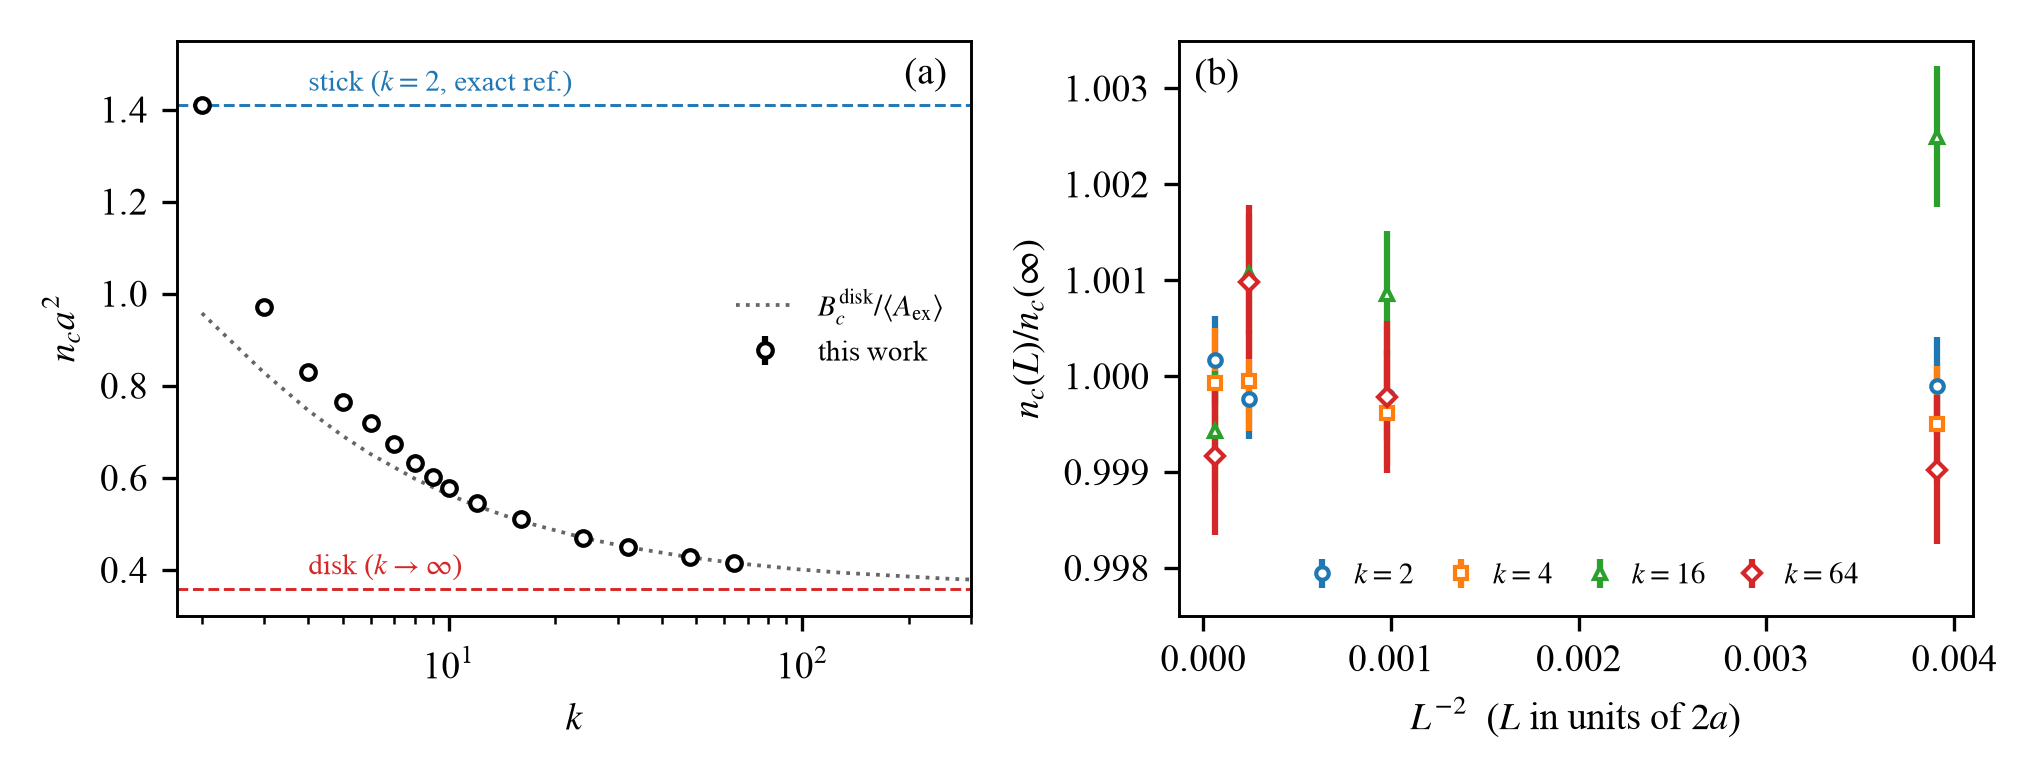
\includegraphics[width=0.86\textwidth]{fig2_threshold.png}
\caption{(a) $n_ca^2$ versus $k$; dashed: stick and disk values; dotted: $B_c^{\rm disk}/\Aex$. (b) Finite-size estimates normalised by the extrapolated value.}
\label{fig:thr}
\end{figure*}

\begin{figure*}[tb]
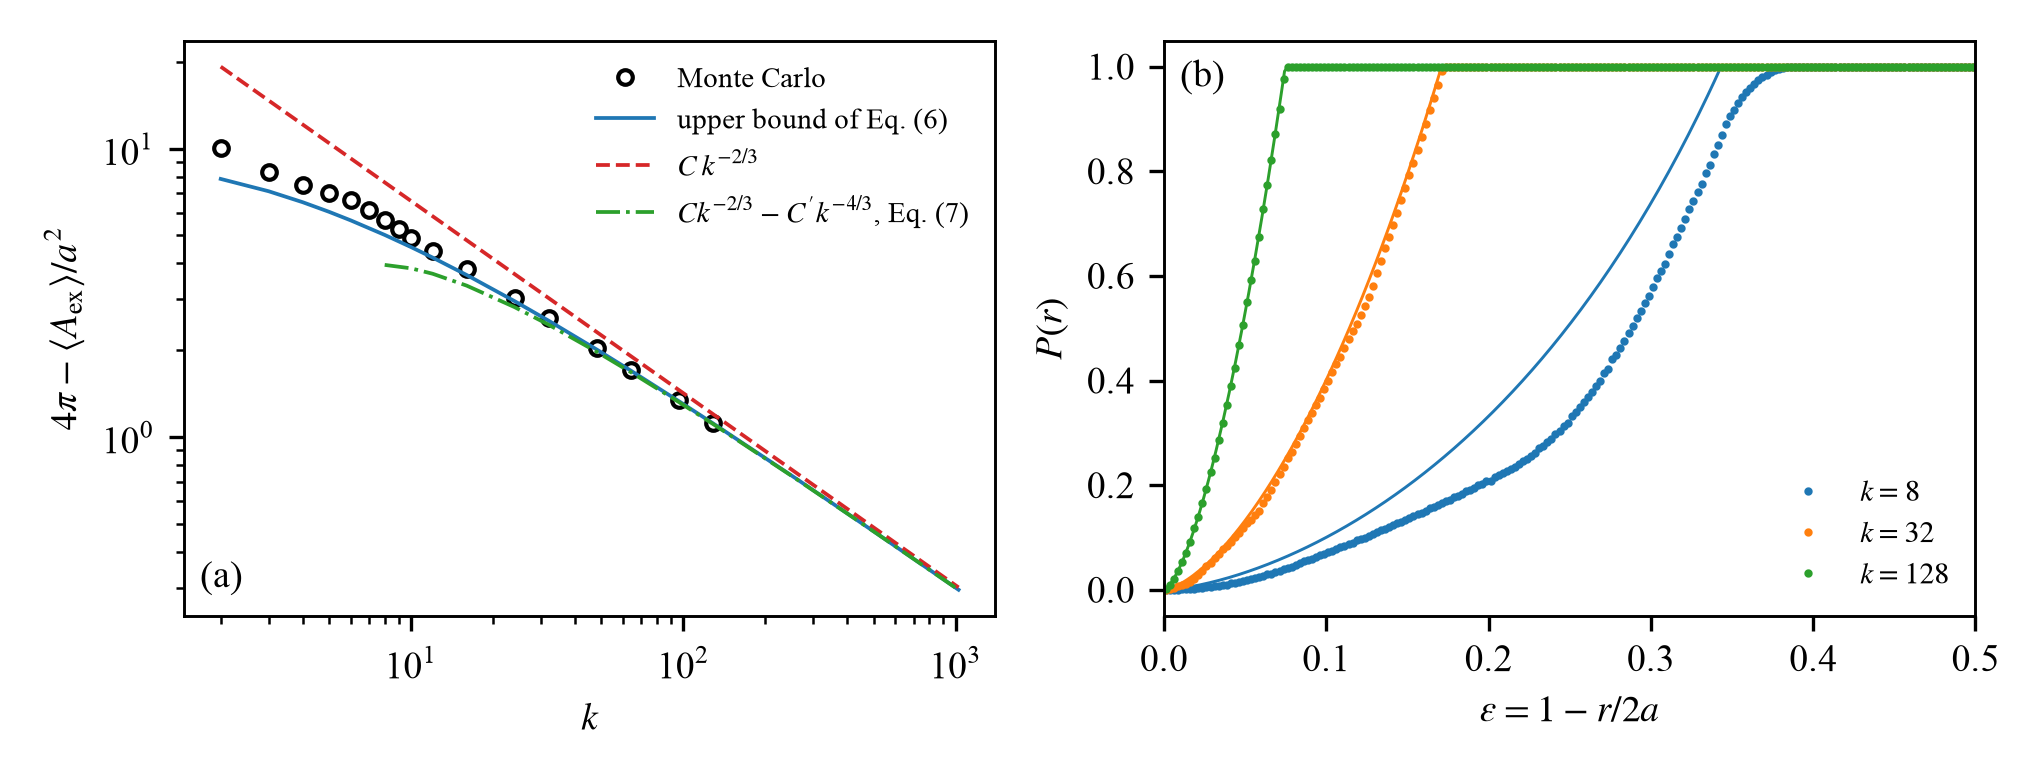
\includegraphics[width=0.86\textwidth]{fig3_excluded.png}
\caption{(a) Excluded-area deficit: Monte Carlo (circles), upper bound of Eq.~\eqref{eq:bounds} (solid), $Ck^{-2/3}$ (dashed), two-term formula~\eqref{eq:thm1} (dash-dotted). (b) Contact probability $P(r)$; points: simulation, lines: upper bound.}
\label{fig:aex}
\end{figure*}

\section{Main theorems}
Let $\varepsilon^*=(h/2c)^{2/3}=(\pi/ck)^{2/3}$.

\begin{theorem}[excluded area]
As $k\to\infty$,
\begin{equation}
4\pi a^2-\Aex=a^2\bigl[Ck^{-2/3}-C'k^{-4/3}+O(k^{-2})\bigr],\label{eq:thm1}
\end{equation}
with $C=\tfrac{18}{5}2^{1/3}\pi^{5/3}\approx30.565$ and $C'=\tfrac{36}{7}2^{-1/3}\pi^{7/3}\approx59.00$.
Explicitly, the $O(k^{-2})$ term is at most $2396/k^2$ for all $k\ge106$.
\end{theorem}
\begin{proof}[Proof sketch]
By monotonicity and~\eqref{eq:bounds}, $P_k=1$ for $\varepsilon\ge\varepsilon_1$, where $\varepsilon_1=\varepsilon^*(1+O(k^{-2/3}))$.
Substituting $\varepsilon=\varepsilon^*t$ into the upper bound gives $P=t^{3/2}(1+\tfrac54\varepsilon^*t+\dots)$, hence $D=8\pi\varepsilon^*[\tfrac35-\tfrac47\varepsilon^*]+O(\varepsilon^{*3})$; the gap between the bounds contributes $\int2\eta/h\,d\varepsilon=O(h^2)$.
Explicit constants are derived in Appendix~\ref{app:rigorous}.
\end{proof}

The exponent $2/3$ has a simple origin: the admissible angular window grows only as $\varepsilon^{3/2}$, so it reaches the arm spacing $h\propto1/k$ at $\varepsilon^*\propto h^{2/3}$.
This is much slower than the $k^{-2}$ convergence of a regular $k$-gon to a disk.

\begin{theorem}[threshold sandwich]
For all $k$, $n_c(k)\ge\nd$. For $k\ge106$,
\begin{equation}
\nd\le n_c(k)\le\nd/(1-\varepsilon_1)^2,\qquad\varepsilon_1\le1.1\,\varepsilon^*,\label{eq:thm2}
\end{equation}
so $0\le(n_c-\nd)a^2\le1.456\,k^{-2/3}(1+o(1))$.
\end{theorem}
\begin{proof}
On a common realisation of centres and orientations, every star lies in the disk of radius $a$ about its centre, so the star graph is a subgraph of the disk graph with connection distance $2a$.
Conversely, by~\eqref{eq:bounds} and monotonicity, stars with centre distance $\le2a(1-\varepsilon_1)$ always touch, so the star graph contains the disk graph with connection distance $2a(1-\varepsilon_1)$, whose threshold is $\nd/(1-\varepsilon_1)^2$ by scaling.
\end{proof}

\begin{conjecture}\label{conj}
$(n_c-\nd)a^2=\dfrac{\eta_cC}{4\pi^2}k^{-2/3}+o(k^{-2/3})$, with $\eta_cC/4\pi^2\approx0.873$; equivalently $B_c(k)=B_c^{\rm disk}+o(k^{-2/3})$.
\end{conjecture}
\noindent\textit{Heuristic argument.}
The star graph differs from the disk graph only through missing edges in the band $2a(1-\varepsilon_1)<r<2a$, missing with probability $1-P_k(r)$.
If the threshold of a connection-function model, $n_c[g]$, were differentiable at the hard-disk function with a sensitivity kernel $K(r)$ continuous at $r=2a$, the change would be $K(2a)D(k)+o(D)$.
Exact scaling of disk radius fixes $K(2a)=\nd/(4\pi a^2)$, which gives the conjecture.
Orientation-induced correlations between missing edges enter only at second order because missing edges are rare.
Neither the differentiability nor the continuity of $K$ is proven for continuum percolation, so we state this as a conjecture.

\section{Numerical results}
\subsection{Thresholds}
Table~\ref{tab:results} and Fig.~\ref{fig:thr}(a) list $n_c$.
For $k=2$ we obtain $1.4095(6)$, in agreement with the exact reference $1.4093215$.
Finite-size effects are below $0.3\%$ for all $k$ [Fig.~\ref{fig:thr}(b)].
$n_c$ decreases monotonically with $k$, and all values lie within the bounds of Theorem~2 (e.g.\ $0.3591\le0.4148\le0.4587$ at $k=64$).

\begin{table}[!ht]
\caption{Critical number density, mean excluded area and critical mean number of contacts. Numbers in parentheses are $1\sigma$ errors in the last digits.}
\label{tab:results}
\begin{ruledtabular}
\begin{tabular}{rlll}
$k$ & $n_ca^2$ & $\Aex/a^2$ & $B_c$\\
\hline
2 & 1.4095(6) & 2.5471 & 3.590(2) \\
3 & 0.9718(6) & 4.2969 & 4.176(3) \\
4 & 0.8294(5) & 5.0937 & 4.225(2) \\
5 & 0.7644(4) & 5.5239 & 4.222(2) \\
6 & 0.7194(5) & 5.9154 & 4.255(3) \\
7 & 0.6740(5) & 6.4148 & 4.324(3) \\
8 & 0.6330(4) & 6.9086 & 4.373(3) \\
9 & 0.6016(5) & 7.3212 & 4.405(3) \\
10 & 0.5780(4) & 7.6537 & 4.424(3) \\
12 & 0.5447(5) & 8.1336 & 4.431(4) \\
16 & 0.5098(5) & 8.7288 & 4.450(4) \\
24 & 0.4701(4) & 9.5288 & 4.479(4) \\
32 & 0.4495(3) & 9.9896 & 4.490(3) \\
48 & 0.4274(3) & 10.5321 & 4.502(3) \\
64 & 0.414792(32) & 10.85312(18) & 4.5018(4) \\
128 & 0.393833(31) & 11.44555(12) & 4.5076(4) \\
256 & 0.380888(30) & 11.84234(8) & 4.5106(4) \\
512 & 0.372792(31) & 12.10263(5) & 4.5118(4) \\

\end{tabular}
\end{ruledtabular}
\end{table}



\begin{figure*}[tb]
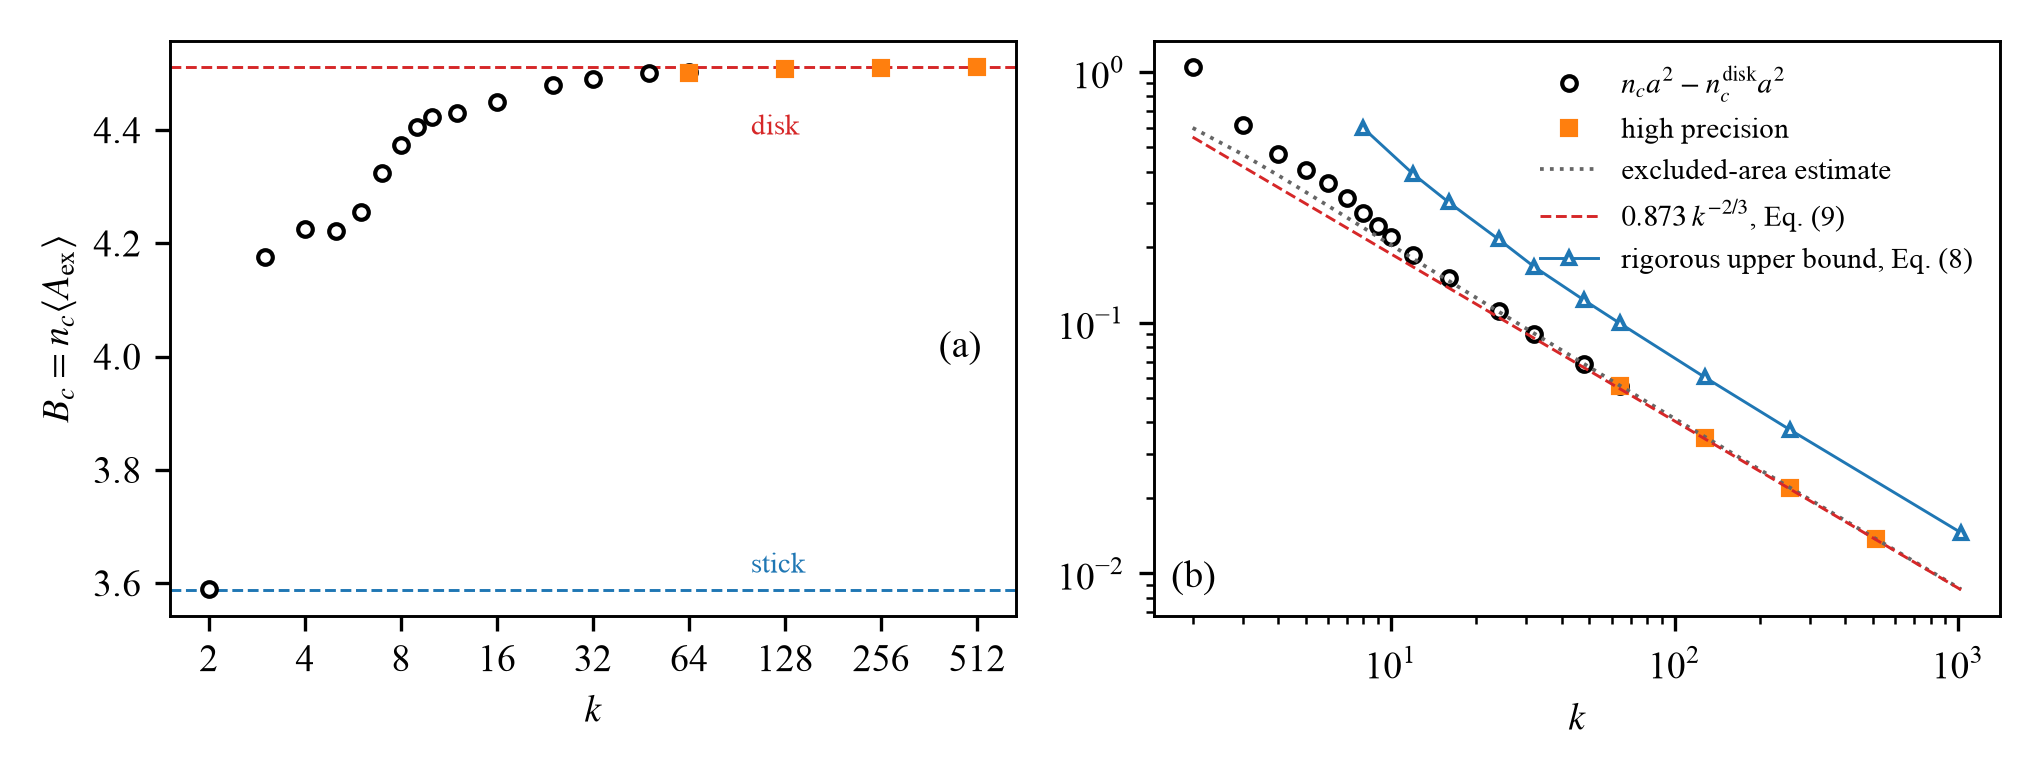
\includegraphics[width=0.86\textwidth]{fig4_Bc.png}
\caption{(a) $B_c=n_c\Aex$; dashed: stick and disk values. (b) $(n_c-\nd)a^2$ with the rigorous upper bound of Theorem~2 (triangles), the excluded-area estimate (dotted) and Conjecture~\ref{conj} (dashed). Squares: high-precision runs.}
\label{fig:bc}
\end{figure*}
\begin{figure*}[tb]
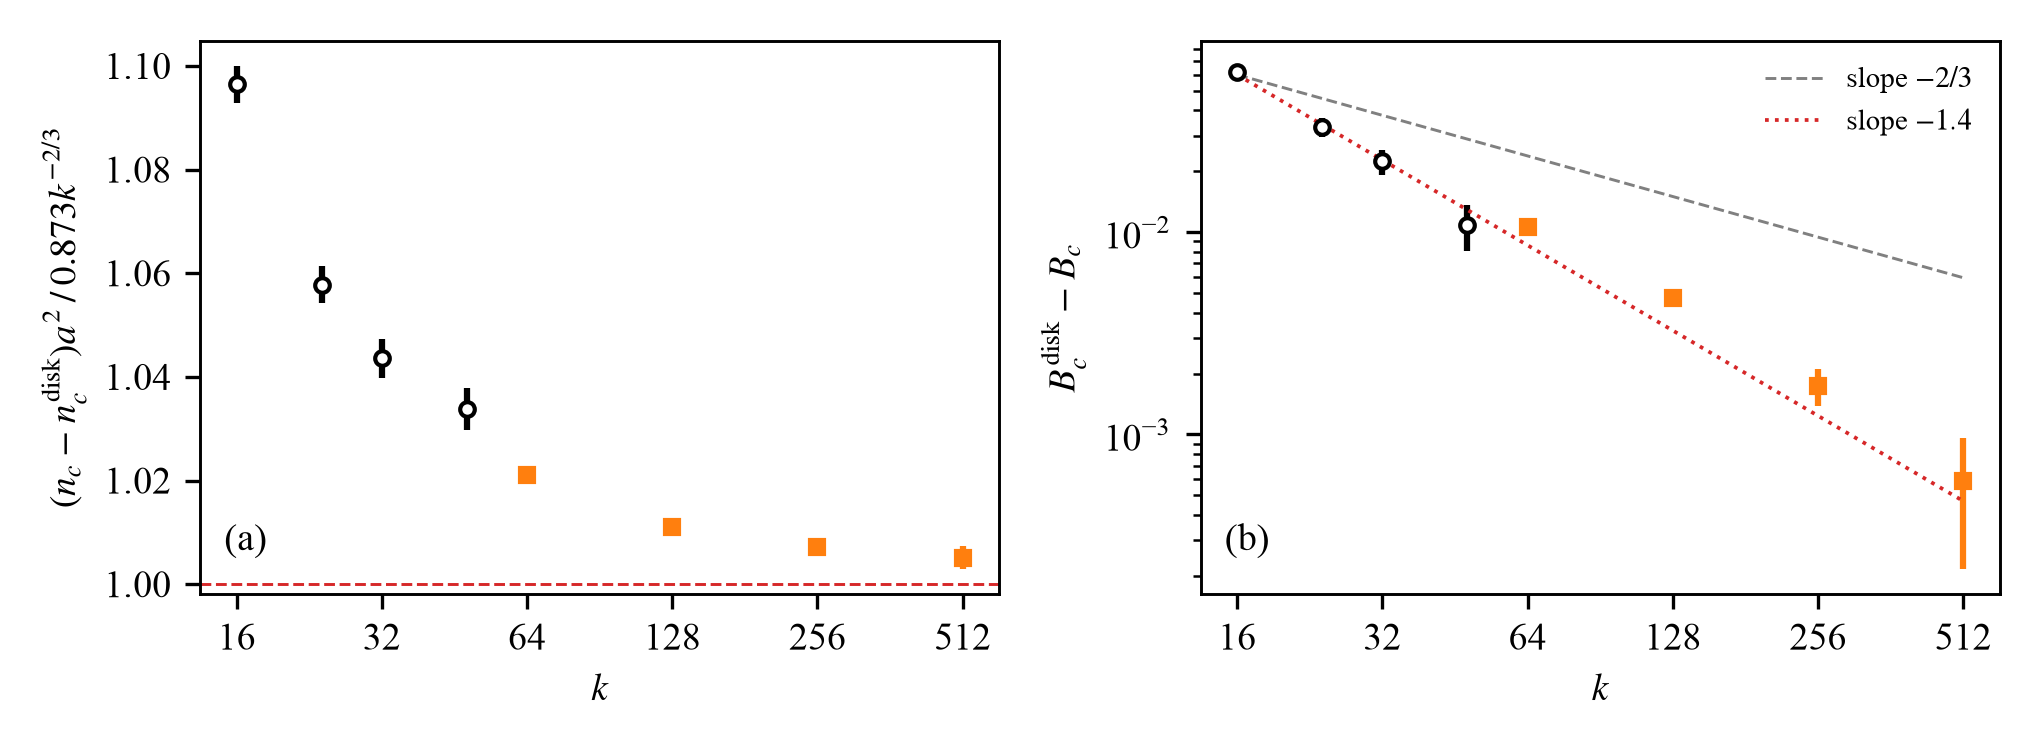
\includegraphics[width=0.86\textwidth]{fig5_conjecture.png}
\caption{Test of Conjecture~\ref{conj}. (a) Measured threshold shift divided by $0.873k^{-2/3}$. (b) $B_c^{\rm disk}-B_c$ with reference slopes.}
\label{fig:conj}
\end{figure*}

\subsection{Excluded area}
Figure~\ref{fig:aex}(a) compares the Monte Carlo deficit $4\pi-\Aex/a^2$ with Theorem~1.
The upper bound in~\eqref{eq:bounds} differs from Monte Carlo by $5\%$, $1.1\%$ and $0.4\%$ at $k=16$, $48$ and $128$.
The two-term formula~\eqref{eq:thm1} matches the upper bound to four digits at $k=512$ and $1024$, whereas the leading term alone is $2\%$ off even at $k=1024$.
High-precision Monte Carlo values for $k\ge128$ (Table~\ref{tab:results}) agree with~\eqref{eq:thm1} within the proven error bound.


\subsection{Critical mean number of contacts and the conjecture}
$B_c$ rises from $3.590$ at $k=2$ (stick value $3.589$) to $4.176$ at $k=3$ and then towards the disk value $4.5123$ [Fig.~\ref{fig:bc}(a)].
It is nearly flat for $k=4$--$6$; additional runs at $k=7,9$ rule out an even--odd effect.
Excluded-area invariance therefore fails by about $25\%$ across the family.
The trend is consistent with the known lowering of thresholds by spread-out connections~\cite{Franceschetti2005}: small-$k$ stars have the broadest $P(r)$.

Figure~\ref{fig:conj} tests Conjecture~\ref{conj}.
The ratio $(n_c-\nd)a^2/(0.873k^{-2/3})$ is $1.021$, $1.011$, $1.007$ and $1.005$ at $k=64$, $128$, $256$ and $512$, approaching unity.
$B_c^{\rm disk}-B_c$ decays roughly as $k^{-1.4}$ ($0.0106$, $0.0047$, $0.0017$, $0.0006$), i.e.\ faster than $k^{-2/3}$, as the conjecture requires.



\section{Discussion}
The contact probability of two regular stars reduces exactly to a lattice-covering problem, which makes the large-$k$ limit tractable and reveals the anomalous $k^{-2/3}$ approach to the disk.
Theorem~2 bounds the convergence rate of the threshold without knowing $\nd$; the prefactor remains conjectural, but the high-precision data support it at the $0.5\%$ level.
Part of the proof of Theorem~1 is computer-assisted and relies on the correctness of the verification program.
Real branched particles have finite arm width and irregular arms; finite width alters near-tangent contacts and may limit the range of $k$ over which the $k^{-2/3}$ law applies.

\section*{Data and code availability}
All code, raw data, the proof note and the computer-assisted verification are available at \url{\RepoURL} under the MIT licence (code) and CC BY 4.0 (data and text).

\section*{Author contributions and use of generative AI}
\ContribEn\
The research design, theoretical analysis, simulation code, data analysis, figures and the manuscript draft were produced with substantial use of a generative AI system (Claude, Anthropic).
The author takes responsibility for the content.

\appendix
\section{Computer-assisted derivation of the explicit constants}\label{app:rigorous}
For $0<\varepsilon\le0.1$ we sandwich $g_\varepsilon$ between explicit functions using
$u-\tfrac23u^3+\tfrac2{15}u^5-\tfrac4{315}u^7\le\tfrac12\sin2u\le u-\tfrac23u^3+\tfrac2{15}u^5$ and
$x+\tfrac{x^3}6+\tfrac{3x^5}{40}\le\arcsin x\le x+\tfrac{x^3}6+\tfrac{3x^5}{40}+R_7x^7$ on $[0,0.55]$, $R_7\le0.05652$.
The support satisfies $\arccos(1-\varepsilon)\le1.43\sqrt\varepsilon$, so all arguments of $\arcsin$ stay below $0.5025$.
After the scaling $\varepsilon=t^2$, $u=tv$, the remainders $(g_\pm/t^3-G_0-t^2G_1)/t^4$ are rational functions, exactly divisible by $t^4$.
We bound them in ball arithmetic (Arb~\cite{Arb}) on a $60\times60$ cover of $[0,1.43]\times[0,\sqrt{0.1}]$.
Combined with $G_0(v)-c=-(v-v_0)^2(v+2v_0)$, this gives
$|\delta_{\max}-c\varepsilon^{3/2}(1+\tfrac54\varepsilon)|\le4.65\,\varepsilon^{7/2}$.
From $g''=2[-2A\sin2u/\sqrt{1-w^2}+wA^2\cos^22u/(1-w^2)^{3/2}]$ with $A=(1-\varepsilon)^{-1}$ and $w=\tfrac A2\sin2u$, we get $g''\le0$ and $|g''|\le21.96\sqrt\varepsilon$.
The integral $F(e)=\int_0^{s_1}(1-es)(1-s^{3/2}-\tfrac54es^{5/2})ds$ satisfies $|F(e)-\tfrac35+\tfrac47e|\le0.799e^2$.
Collecting terms gives the constant $2396$ and the covering condition for $k\ge106$.
Direct numerics give $2.01$ and $10.46$ for the quantities bounded by $4.65$ and $21.96$.

\begin{thebibliography}{99}
\bibitem{Stauffer1994} D. Stauffer and A. Aharony, \textit{Introduction to Percolation Theory}, 2nd ed. (Taylor \& Francis, 1994).
\bibitem{Balberg1984} I. Balberg, C. H. Anderson, S. Alexander, and N. Wagner, Phys. Rev. B \textbf{30}, 3933 (1984).
\bibitem{Mertens2012} S. Mertens and C. Moore, Phys. Rev. E \textbf{86}, 061109 (2012).
\bibitem{Baker2002} D. R. Baker, G. Paul, S. Sreenivasan, and H. E. Stanley, Phys. Rev. E \textbf{66}, 046136 (2002).
\bibitem{Pike1974} G. E. Pike and C. H. Seager, Phys. Rev. B \textbf{10}, 1421 (1974).
\bibitem{Li2013} J. Li and M. \"Ostling, Phys. Rev. E \textbf{88}, 012101 (2013).
\bibitem{Manna2003} L. Manna, D. J. Milliron, A. Meisel, E. C. Scher, and A. P. Alivisatos, Nat. Mater. \textbf{2}, 382 (2003).
\bibitem{Geigenfeind2019} T. Geigenfeind and D. de las Heras, J. Chem. Phys. (2019), doi:10.1063/1.5092865; arXiv:1902.05961.
\bibitem{RoyTanemura2002} R. Roy and H. Tanemura, Adv. Appl. Probab. \textbf{34}, 48 (2002).
\bibitem{NewmanZiff2001} M. E. J. Newman and R. M. Ziff, Phys. Rev. E \textbf{64}, 016706 (2001).
\bibitem{Pinson1994} H. T. Pinson, J. Stat. Phys. \textbf{75}, 1167 (1994).
\bibitem{Numba} S. K. Lam, A. Pitrou, and S. Seibert, in \textit{Proc. 2nd Workshop on the LLVM Compiler Infrastructure in HPC} (2015), p.~1.
\bibitem{Franceschetti2005} M. Franceschetti, L. Booth, M. Cook, R. Meester, and J. Bruck, J. Stat. Phys. \textbf{118}, 721 (2005).
\bibitem{Arb} F. Johansson, IEEE Trans. Comput. \textbf{66}, 1281 (2017).
\end{thebibliography}

\end{document}
